\documentclass[10pt]{exam}
\usepackage[phy]{template-for-exam}
\usepackage{graphicx}
\usepackage{caption}

\title{Reflection Lab}
\author{Rohrbach}
\date{\today}

\begin{document}
\maketitle

\noindent
{\small \it This lab is based on Experiment \#2 in PASCO's Introductory Optics System Manual and images are borrowed from it.}

\section*{Purpose} To observe what happens to rays of light as they reflect off a plane mirror.

\noindent
\begin{figure}[h]
  \centering
  \begin{minipage}[b]{10cm}
    \centering
    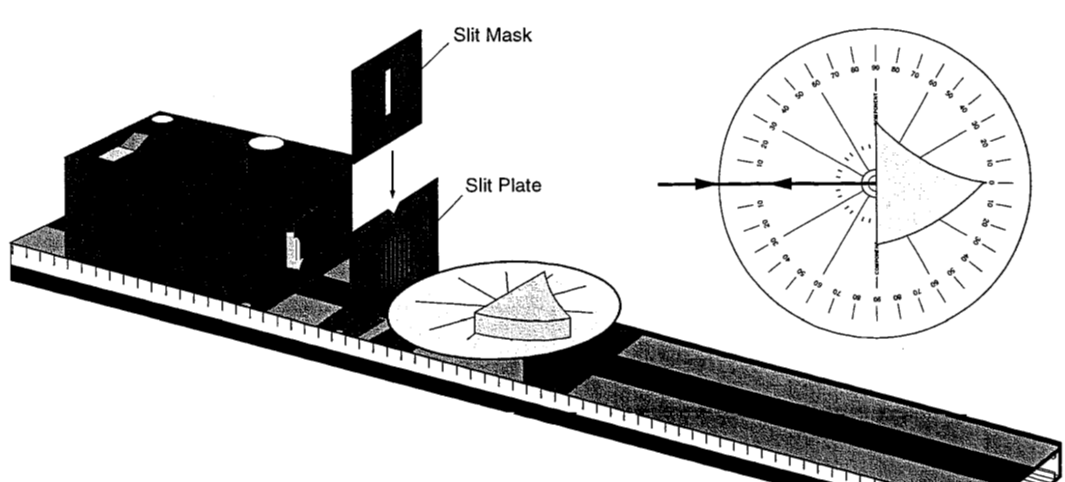
\includegraphics[width=8cm]{Fig2_1.png}
    \captionof{figure}{Equipment Setup}
    \label{fig:equip}
  \end{minipage}%
  \begin{minipage}[b]{6cm}
    \centering
    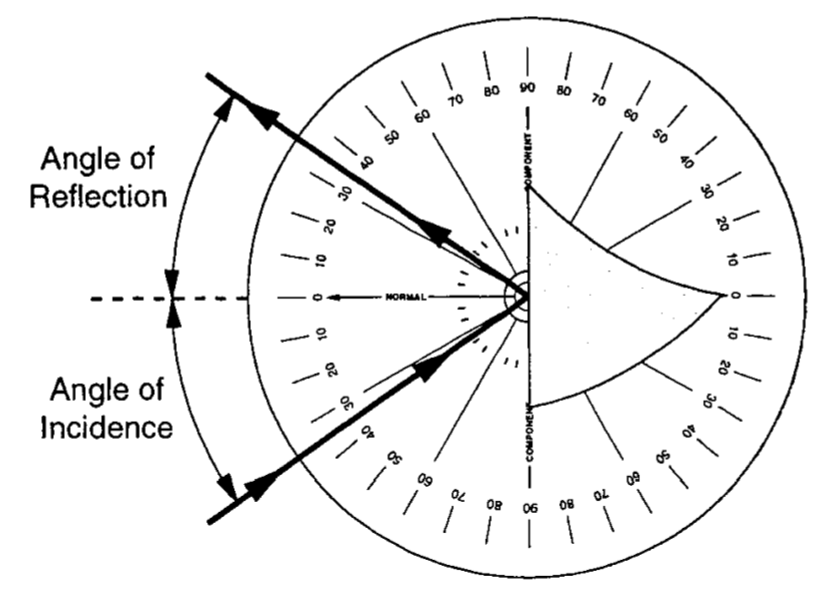
\includegraphics[width=4.5cm]{Fig2_2.png}
    \captionof{figure}{Incident and Reflected Rays}
    \label{fig:rays}
  \end{minipage}
\end{figure}

\vspace{-1em}

\section*{Procedure}
\begin{enumerate}
  \item Set up the experiment as indicated in Figure~\ref{fig:equip}.
  \item Adjust the components so that a single ray of light is aligned with the bold arrow labeled “normal” on the Ray Table Degree Scale.
  \item Carefully align the flat part of the mirror along the bold arrow labeled “component” on the Ray Table Degree Scale.
  \item Rotate the Ray Table so that the Angle of Incidence (see Figure~\ref{fig:rays}) changes.  Record the angle of reflection.
  
\end{enumerate}

\section*{Data} \hfill

\vspace{1em}

\renewcommand{\arraystretch}{1.6}

\begin{tabular}{|c|c|c|}
  \hline
  Angle of incidence &
  Angle of reflection &
  Angle of reflection \\
  &
  (when incidence is \emph{above} normal line) &
  (when incidence is \emph{below} normal line) \\\hline
  $10^\circ$ && \\\hline
  $20^\circ$ && \\\hline
  $30^\circ$ && \\\hline
  $40^\circ$ && \\\hline
  $50^\circ$ && \\\hline
  $60^\circ$ && \\\hline
  $70^\circ$ && \\\hline
  $80^\circ$ && \\\hline
\end{tabular}

\begin{questions}

\uplevel{\section*{Analysis}}

  \question
    Are the results of the two trials (above normal line and below normal line) the same?  If not, to what do you attribute the difference? \vs[2] 

  \question
    What relationship seems to hold between the angle of incidence and the angle of reflection \vs[2] 

  \question
    Why was it helpful to do both trials (above and below the normal line)?  Why was this better than just doing the one above the normal line? \vs[2] 

\uplevel{
  \section*{Reading Questions}
  \emph{All information is found in the reading attached to this page.}
}

    \question
      Define each of the following:

      \begin{parts}
        \part normal \vs
        \part angle of incidence \vs 
        \part angle of reflection \vs
      \end{parts}
    
    \question
      What is the law of reflection? \vs[2]
    
    
    \question
      Do all surfaces reflect light, and if so, why can a reflection only be seen in certain objects? (\emph{Hint:} try reading about \emph{diffuse reflection}) \vs[2]
    
    \question
      How is it possible that the satellite dish shown in Figure 28.11 is cosnsidered ``polished''? \vs[2]

\end{questions}




\end{document}